\chapter{Background}
Creating a cyborg is a massive cross disciplinary effort, and if a scope is not
clearly defined the background runs the risk of becoming equally massive.
The goal of the thesis is to create a hybrid neuro-digital system capable of
controlling a simple robot, and by extension to create a ``bridge'' between
neural and digital.
Each section in the background shares this bridge as a red thread, and
consequently topics that are not directly related to the thesis' goal are discarded.
The background is laid out as follows:
First \emph{Complex Systems} are introduced as a framework to discuss the computational
capabilities in a wide range of systems that exhibit system dynamics similar to
that of neurons.
Modeling neurons as a complex systems is a first step towards establishing a
common ``language'' between neural activity and digital logic.
%
Next, \emph{Evolution in Materio}, EiM for short, introduces computation done in
unstructured matter through the process of evolution.
The goals of EiM are closely aligned to the goal of this thesis, as both study
massively parallel computation happening in physical matter shaped by the
process of evolution.
%
Next section, \emph{Neurons As Computers} introduces neurons with a strong focus
on their computational capabilities.
Building on the EiM section, this section motivates a necessary reduction of
scope, proposing a simplified model of the computing neuron and a medium of
communication between neuron and digital.
%
Finally, \emph{Reservoir Computing} is introduced, tying together the previous
sections by introducing the framework of reservoir computing in order to
establish a common ``language'' between neural cultures and digital.
\section{Complex Systems}
% TODO: Introduser Adaptive networks, siter Sayama: "Modeling complex systems with
% adaptive networks"\\ \\
%
Nature, unlike humans, does not shy away from complexity.
On all scales, from entire ecosystems and social networks, anthills, neural
tissue and the gene regulatory networks in single cells nature exhibits dizzying
complexity.
%
Unlike a swiss watch which consists of many complex parts that operate in a
simple way, these system exhibit complexity in their \emph{interactions}.
%
From an evolutionary standpoint this makes sense.
A system whose behavior rises from interaction is less dependent on each
individual part, giving rise to robust systems that can adapt to change.
Robustness is necessary for evolution to because it provides a \emph{fitness
landscape} that evolution can ``maneuver''.
%
From a systems perspective the brain has much more in common with an anthill
than a processor, to understand neural cultures a good first step is to look at
other systems with complex interaction.\par
%
%
The study of these \emph{Complex Systems} is a broad, cross-disciplinary field,
not restricted to biological systems.
%
In [cite Bar Yam Dynamics of complex systems] Bar-Yam suggests that complex
systems is a convergence point for all disciplines that deal with systems as
shown in \ref{figBarYam}.
%
All of these fields feature systems in which the global behavior \emph{Emerges}
from local interaction of individual components through a process of \emph{Self
  Organization}.
These behavior of these systems exhibit a complexity that is greater than the
sum of complexity of its individual components, i.e the relationship between the
complexity of the system and its constituent components is \emph{Non Linear}.
Common for these systems is therefore the futility of reductionism since the
interesting aspects of the system only occurs when components interact.
It is difficult to pin down exactly what a complex system is, so before
venturing further a practical example is in order.
\begin{figure}[h!]
  \centering
  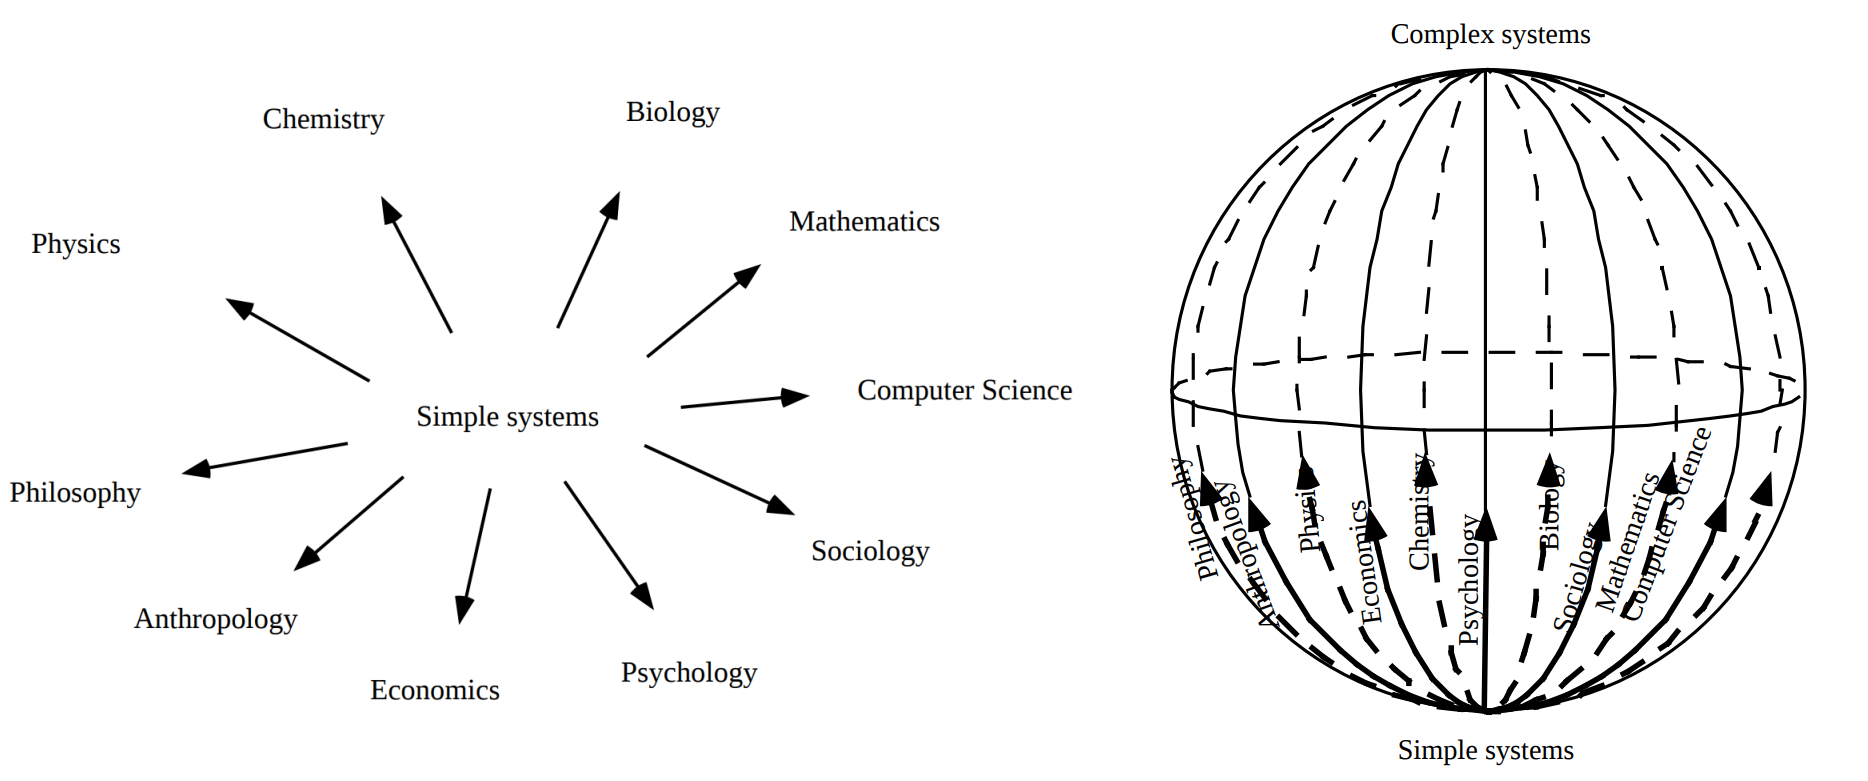
\includegraphics[width=1\textwidth]{fig/BarYamCX.png}
  \caption{From Bar Yam book.}
  \label{figCX}
\end{figure}
\subsubsection{Cellular Automata}
A \emph{Cellular Automaton}\footnote{Singular: Automaton, Plural: Automata}
is a simple discrete model of a single cell which changes between a discrete set
of states based only on its immediate neighbors.
Figure \ref{figCA22} shows an example of a \emph{rule set}, or \emph{transition
  table} for a cellular automaton with only two states which over several step
forms a pattern.
Clearly some global behavior emerges from local interaction, do all transition
tables lead to complex systems?
%
Stephen Wolfram suggests classifying the behavior of cellular automata into four
classes [cite wolfram yo]:
\begin{description}
\item [Class I] evolves to a homogeneous state.
\item [Class II] evolves to simple separated periodic structures.
\item [Class III] yields chaotic aperiodic patterns.
\item [Class IV] yields complex patterns of localized structures
\end{description}
%
The behavior shown in \ref{figCA22} fits in the second category, outside of the
complex category, so clearly self organization is not enough.
%
In Langton's pioneering paper \emph{Computation on the Edge of Chaos}
\cite{langton_computation_1990} the space of possible transition tables for one
dimensional cellular automata with two states, such as \ref{figCA22} is explored.
For each transition table Langton calculated the ratio of states that lead to
``death'' to ``life'' (white and black cell respectively).
\begin{figure}[h!]
  \centering
  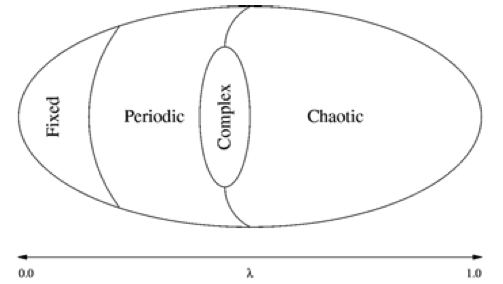
\includegraphics[width=1\textwidth]{fig/Langtons_egg2.png}
  \caption{Langtons egg}
  \label{figCAegg}
\end{figure}


the system dynamics of cellular automata are shown to follow phase transitions
similar to physical matter.
Langton explored the rule space of cellular automata and found that the ratio
between transitions that led to cell death and life had similarities to
temperature in physical systems.
As expected, rules which tended to favor cell death led to static or periodic
systems, while rules favoring life over death led to chaotic systems.
More interstingly is what happened when the rules favored life and death
equally.
In these systems which exists at the border between orderly and chaotic systems
Langton found a \emph{critical} phase where the system was neither chaotic nor
ordered.


Together they are capable of solving global problems such
as contour-extraction \cite{sipper_emergence_1999}, providing an example of
local interactions producing interesting global behavior.\par
Cellular automata are even sufficiently powerful to express a turing machine,
but as Sipper puts it: ``This is perhaps the quintessential example of a slow
bullet train: embedding a sequential universal Turing machine within the
highly parallel cellular-automaton model.''
Embeddeding turing machines into cellular automatas is of little use, but it's
useful to know that cellular automata are sufficiently powerful if we are to
apply it as a model for the processes governing neural networks.
The real power of cellular automatas as a model for neural networks is how they
model the \emph{Phase Transitions} in behavior (i.e dynamics).


% Langton burde faktisk komme inn allerede her.
Unlike chaotic systems, complex systems contain \emph{Attractors}, states that
are relatively stable.
Fig [Strange attractor] shows the \emph{Strange Attractor}, a pattern formed by
a particle in a vector field that orbits two attractors, arbitrarily switching
between them.
In complex systems both dampening and amplifying feedback loops form.
The dampening loops allow the system to fall into the attractors, while the
amplifying loops can amplify minor perturbations, eventually causing a cascading
feedback loop moving the system to a different attractor.\par
%
%
%
% The immediate benefit of classifying neural cultures as a complex systems is
% that studying simpler models of complex systems can act as a stepping stone.
% A simple, biological inspired model capable of exhibiting complex behavior is
\begin{figure}[h!]
  \centering
  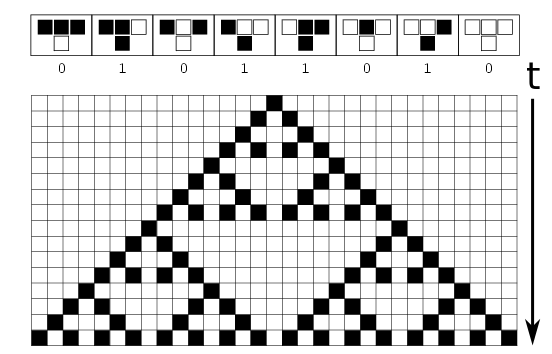
\includegraphics[width=1\textwidth]{fig/ca22.png}
  \caption{Should add a time axis to drive the point home that these are 1D}
  \label{figCA22}
\end{figure}
the \emph{Cellular Automaton}, a discrete model of a single cell which changes
between a discrete set of states based only on its immediate neighbors.
Together they are capable of solving global problems such
as contour-extraction \cite{sipper_emergence_1999}, providing an example of
local interactions producing interesting global behavior.\par
Cellular automata are even sufficiently powerful to express a turing machine,
but as Sipper puts it: ``This is perhaps the quintessential example of a slow
bullet train: embedding a sequential universal Turing machine within the
highly parallel cellular-automaton model.''
Embeddeding turing machines into cellular automatas is of little use, but it's
useful to know that cellular automata are sufficiently powerful if we are to
apply it as a model for the processes governing neural networks.
The real power of cellular automatas as a model for neural networks is how they
model the \emph{Phase Transitions} in behavior (i.e dynamics).
In Langton's pioneering paper \emph{Computation on the Edge of Chaos}
\cite{langton_computation_1990}
the system dynamics of cellular automata are shown to follow phase transitions
similar to physical matter.
Langton explored the rule space of cellular automata and found that the ratio
between transitions that led to cell death and life had similarities to
temperature in physical systems.
As expected, rules which tended to favor cell death led to static or periodic
systems, while rules favoring life over death led to chaotic systems.
More interstingly is what happened when the rules favored life and death
equally.
In these systems which exists at the border between orderly and chaotic systems
Langton found a \emph{critical} phase where the system was neither chaotic nor
ordered.
It is important to note that Langton did not seek to solve a specific problem
with his automatons, but to explore which automatas capable of supporting
universal computation, hypothesized by Wolfram \cite{wolfram_universality_1984}.
Criticality applies to any dynamic system, not just cellular automata, and the
study of adaptive networks \cite{sayama_modeling_2013} suggests that many
systems exhibit a homeostatic regulation of system dynamics to ensure that it
stays in the critical phase, including neurons
\cite{bornholdt_topological_2000}.

\section{Evolution In Materio}
Classifying neurons as a complex system has not gotten us closer to a solution
for interfacing with them in a meaningful way it seems.
However, one useful conclusion is that neurons work nothing like human designed
conventional computers, and that to understand how neurons compute we should
look at more \emph{unconventional computing}, specifically work done on physical
matter.
Two pioneers in this field were the british duo Pask and Beer which studied how
unstructured matter could be used to perform computational tasks.
In the introduction Toffolis statement that computation does not make sense
except in the light of evolution seems to contradict this notion of computation,
but evolution is not reserved only for nature.

% TODO: Cite
In one experiment [cite ???] the duo used silver in an acidic solution which would form
short-lived silver filaments when subjected to electric currents.
From our perspective of computation, it was not before they tuned the parameters
of the system in order to evolve a tone discriminator that the system could
truly be classified as a computing one.
Evolution in materio represents a very different approach than conventional
processors.
While it is impossible to program unstructured matter with imperative
instructions like in a conventional computer, we can nonetheless ``instruct''
the material computer in a declarative matter by specifying what sort of result
we are after and letting the evolutionary process handle the rest.
Material computing gives us a much better model of how neurons can compute:
Material computation happens on a massively parallel scale, it occurs in a
substrate where all structure is self-organized rather than imposed by a
designer, and both are products of evolution.\\

TODO: Write about Odd Rune's stuff, clean up and add citations.

\section{Neurons As Computers}
It might seem that the previous section has provided the key to unlocking the
computational power of neural cultures.
This line of thinking neglects the fact that neurons have already been shaped by
the process of evolution over billions of years, indeed neural cultures can be
viewed as the result of an EiM experiment a billion years in the making.
Our goal is not to apply the principle of EiM to neural cultures, but it does
provide an interesting angle:
When Pask and Beer tweaked their silver solution to discriminate tones, they did
viewed the solution as a black box, and only its performance on the task at hand
was evaluated.
While evolution does not optimize for a specific functionality the black box
approach is similar.
Just like Pask and Beer did not consider the exact inner workings of silver
filaments, it is necessary to apply the black box liberally when approaching
neurons.

% I really like the gist of this, but I'm very unsure about the phrasing.
If the neuron was the result of an EiM experiment, the ideal model of the neuron
would be the criteria used to evaluate fitness, eschewing all implementation
details.
Of course, no such criterias exist, evolution does not have a plan, but it
illustrates why as much as possible of the cells inner working will be
considered to be inside a black box.

% Another thing missing is of course how to utilize neurons.

\subsection{Neurons}
The neuron, or nerve cell, is the basic building block of both the human brain
and the nerve system.
There are many types of neurons in the human body, but to reduce the scope the
focus of this thesis is a simplified model of the neurons that make up the
brain.
The model neuron, shown in fig [a figure of a neuron] consists of three parts:
The body, \emph{Soma}, the \emph{Dendritic network} and an \emph{Axon}.
The dendritic network acts as a receptor sensing electrical activity around the
neuron, while the axon transmits electric pulses to neighboring cells.
The connection between two neurons is called a \emph{Synapse}.
Axons and dendritic networks are themselves vastly complex, and viewing them as
simple electrical transmitters neglects the importance of neurotransmitters.
However, given the strong correlation between neurotransmitter concentrations and
electrical activity is considered part of the black box.
When the neuron is sufficiently excited by electrical activity it will fire an
electrical pulse that travels along the axon, which in turn stimulate other
neurons.
Together neurons form networks in a complex interplay between topology and behavior:
The behavior of the network decides its behavior, and the behavior in turn
causes some synapses to wither, and others to form in a process that is not well
understood.
The model used for the neuron for the rest of this paper is a node in an
\emph{Adaptive Network} which communicates through electrical pulses.
The missing part in our model is the underlying rules that dictates the growth
of the network.
% What about spike trains?
\section{Reservoir Computing}
So far we have arrived at a model of the neuron as a complex adaptive network
which can be interfaced with using electrical signals, but the fundamental issue
of actually utilizing neurons for computing remains.
%
The final piece of the puzzle comes in the form of \emph{Reservoir Computing}, a
technique developed to exploit the dynamics of complex systems.
If the fundamental rule governing the neuron is to create networks exhibiting
the same complexity behavior as Langton's automatas then harnessing the
computational capabilities of these simple models is a first step towards
interfacing and understanding neurons.
%
% Clearly designing a cellular computer in a top down manner is intractable due to
% the intricate and unpredictable relation between cause and effect.
% The best we could realistically achieve with the typical top down approach is
% implementing a turing machine which would be both slow and incredibly brittle.
% Seemingly, classifying the neural culture as a complex system has not provided
% any useful tools for understanding how to interact with it, on the other hand it
% makes this task seem futile.
% However, in computer science the recent field of
% \emph{reservoir computing} has emerged, embracing the complexity and unpredictability
% of certain complex systems.
In reservoir computing, a complex systems is used as a \textit{reservoir}
\cite{schrauwen_overview_2007} which
``acts as a complex nonlinear dynamic filter that transforms the
input signals using a high-dimensional temporal map, not unlike the operation
of an explicit, temporal kernel function.''\\
% cite on SVMs?
In order to explain, schrauwen makes a comparison to the the machine learning
technique of source vector machines work, as shown in fig [rm 1]:
The reservoir acts as a kernel, projecting input into a high-dimensional feature space.
Figure [rm 1] shows this technique, note that the regression performed upon the
feauture space is a simple linear regression, an important point both in SVMs
and reservoir computing.
%
Figure [rm 2] shows a typical reservoir computing setup which follows a similar
method of operation as the SVM in figure [rm 1]
The reservoir serves as the high dimensional feature space, while the output
layer is only capable of linearly separating the resulting dynamics.
%
Schrauwen points out two major differences between SVMs and RCs.
First, SVMs only implicitly expands the input to high dimensional space in order
to make the problem tractable, while reservoirs do not.
Secondly, kernels are not capable of handling temporal signals.
%
The second difference is very important, it is what allows reservoirs to
implicitly encode temporal signals in their dynamics, making reservoirs a
natural fit for tasks such as speech recognition.
% cite Biologically Plausible Speech Recognition with LSTM Neural Nets Alex
% Graves, Douglas Eck, Nicole Beringer, Juergen Schmidhuber
% 
In other terms, the properties that make complex systems so hard to work with
such as sensitivity to initial conditions also allow them to discern very subtle
nuances in input, and their complex behavioral patterns causes the systems to
change their behavior to new input based on previous input.
%
In light of this, asking how to build a computer using Langton's automatons is
the wrong question, instead the focus should be on how exploit the computation
that is already occuring.\\
There are many examples of reservoirs which have been successfully exploited:
In \cite{jaeger_adaptive_2003} an \textit{echo state network} 
is utilized to solve classification problems.
More esoteric reservoirs have been used, for instance in
\cite{natschlager_liquid_2002} the idea of reservoir computing is taken quite
literally using a bucket of water as a reservoir.\\

\subsection{Linear and nonlinear output layers}
TODO: Elaborate on the use of linear vs nonlin classifiers.

\cleardoublepage

%%% Local Variables:
%%% mode: latex
%%% TeX-master: "../main"
%%% End: